% -*- mode: fundamental -*-

% ****************************************************************

\chapter{BSV: FSMs; \\
RISC-V: the Drum unpipelined CPU}

\markboth{Ch \arabic{chapter}: The Drum CPU (DRAFT)}{\copyrightnotice}

\setcounter{page}{1}
% \renewcommand{\thepage}{\arabic{page}}
\renewcommand{\thepage}{\arabic{chapter}-\arabic{page}}

\label{ch_Drum_FSMs}

% ****************************************************************

\section{Introduction}

So far, we have only been discussing pure combinational functions, for
which there is no concept of time.  Combinational functions are just
pure mathematical functions, ``instantaneously'' transforming input
values to output values.  However, a CPU, as shown in
Figure~\ref{Fig_Drum_Instr_Exec}
\begin{figure}[htbp]
  \centerline{\includegraphics[width=6in,angle=0]{ch030_RISCV_Design_Space/Figures/Fig_Instr_Exec_w_structs}}
  \caption{\label{Fig_Drum_Instr_Exec}
           Simple interpretation of RISC-V instructions
	   (same as Fig.~\ref{Fig_Fetch_function_Simple_Instr_Exec})}
\end{figure}
represents a \emph{processs}, a behavior that evolves over time.  For
example the Drum CPU executes one full instruction after another, and
the black arrows in the diagram represent an infinite loop. For each
instruction, first it performs a Fetch operation, which sends a
request to memory. Some time later, the memory sends back a response,
which is then processed by the Decode step, Register-Read-and-Dispatch
step and then one of the Execute steps.  The Execute Memory Ops step
sends a request to memory. Some time later, the memory sends back a
response, which is processed in the Retire step.  Finally, it it loops
back to the Fetch step, and the process repeats for the next
instruction.

The simplest temporal process in hardware is the FSM (Finite State
Machine).  Figure~\ref{Fig_Drum_Instr_Exec} can be interpreted as an
FSM: each yellow rectangle is a state, and the process transitions
from state to state, thereby executing RISC-V instructions.  This is
exactly what the Drum CPU does.  In this chapter, after first
discussing FSMs in BSV, we discuss the Drum CPU and its FSM
implementation.  By the end of this chapter, we will have a complete
Drum CPU that is capabable of executing RV32I RISC-V programs.

% ****************************************************************

\section{BSV: Finite State Machines (FSMs)}

\label{Sec_FSMs_FSMs}

\index{BSV!FSMs}
\index{BSV!Finite State Machines}

Finite state machines (FSMs) are a classical concept in digital
hardware design, representing a hardware \emph{process}.  An FSM is an
artefact that can, at any time, be in one of a number of possible
\emph{states}.  One state is often distinguised as the \emph{start}
state, the initial state of the FSM.  From each state, an FSM can
\emph{transition} to another state; the choice of destination state
may depend on predicates on the current state and on external inputs
to the FSM.

One classical notation for FSMs is the ``bubble-and-arrow'' diagram: a
bubble represent a state, and arrows between bubbles represent
transitions between states.  Thus, an FSM is a specification of a
process that, over time, moves from state to to state.  The process
can loop infinitely, with transitions back to earlier states.

In classical notation, arrows may be annotated with \emph{c/o} labels
(conditions and outputs).  The condition on an arrow indicates under
what conditions this transition is taken, usually a (pure) boolean
predicate on the current state and external inputs.  A state may have
arrows to multiple next-states, with mutually exclusive conditions,
thus expressing an if-then-else situation.\footnote{If the conditions
are not mutually exclusive, we have a so-called
\emph{non-deterministic} FSM, where the next-state is chosen
non-deterministically from all true conditions on outgoing arrows.  In
hardware design and in this book we are only concerned with
deterministic FSMs, where the outgoing conditions will be mutually
exclusive and we always have a deterministic, unique next-state.}  The
outputs on an arrow represent external outputs driven by the FSM
starting with that transition and until the next transition.  An arrow
without a condition is an unconditional transition to the next-state.
An arrow may also omit an output.

\index{Drum!as an FSM}

For Drum, we will interpret Figure~\ref{Fig_Drum_Instr_Exec} as a
bubble-and-arrow diagram for an FSM.  Each of the yellow ``bubbles''
is a state, and the black arrows represent state-transitions.  We will
not annotate the arrows with labels, leaving the reader to refer to
the BSV code.

% ================================================================

\subsection{Sequential FSMs, Concurrent FSMs, and Digital Hardware}

\index{BSV!FSMs!sequential {\vs.} concurrent}
\index{BSV!FSMs!concurrent {\vs.} sequential}

Classical FSMs in the literature are \emph{sequential} FSMs---every
transition is from the current state to a unique, particular next
state.\footnote{Even in non-deterministic FSMs, though there may be
several possible next-states, exactly one next-state is
non-deterministically chosen.}

Most non-trivial digital hardware systems are actually
\emph{concurrent FSMs}, {\ie} multiple classical FSMs running
concurrently and independently and interacting with each other.
Different BSV module instances are separate FSMs, each running their
own process(es).  These separate FSMs may communicate with each other
{\via} shared state (registers, fifos, register files, {\etc}).

\index{Fife!as a set of concurrent FSMs}

For Fife, we will interpret Figure~\ref{Fig_Drum_Instr_Exec} as a set
of concurrent FSMs.  Each of the yellow boxes in the figure will be a
separate module containing zero or more concurrent FSMs, and the black
arrows represent communication between FSMs.

% ****************************************************************

\section{BSV: {\tt StmtFSM}}

\label{Sec_FSMs_StmtFSM}

\index{BSV!StmtFSM@{\tt StmtFSM}}

The central BSV construct for temporal behavior (processes) is the
``\verb|rule|''.  Collections of rules can express any sequential or
concurrent FSM.  However, because Drum is a simple, structured
sequential process, we can use a simpler, higher-level BSV notation
called ``\verb|StmtFSM|'' (which, in turn, is just converted into
rules by the \emph{bsc} compiler).

\verb|StmtFSM| is a sub-language within BSV which is suitable for
expressing \emph{structured} sequential processes.\footnote{{\tt
StmtFSM} can also express structured fork-join concurrency, but we do
not need that capability for Drum.}  By ``structured'' we mean that
processes are constructed by composing construct similar to those in
most common sequential programming languages: blocks to express
temporally sequenced actions, if-then-elses, while-loops and
for-loops.

% ----------------
\vspace{2ex}

NOTE:
\fbox{\small
\begin{minipage}{5in}

We already briefly encountered a simple {\tt StmtFSM}, with just a
sequential block, in the testbench in
Section~\ref{BSV_small_testbench}.

\end{minipage}}
% ----------------

% ================================================================

\subsection{Actions and the {\tt Action} type}

\index{BSV!Action@{\tt Action}: primitive type of actions}
\index{BSV!actions}

The fundamental building-block for \verb|StmtFSM| is the ``action'',
which is a statement/expression of type \verb|Action|.  Some common
examples:

{\small
\begin{Verbatim}[frame=single, numbers=left]
   rg_pc <= rg_pc + 4;          // Assignment to a register
   f_F_to_D.deq;                // Dequeue a fifo
   f_D_to_RR.enq (v);           // Enqueue into a fifo
   $display ("Hello, World!");  // Print something (in simulation only)
\end{Verbatim}
}

As discussed in
Section~\ref{Sec_Register_syntactic_shorthands}
the first assignment statement is syntactic shorthand for:

{\small
\begin{Verbatim}[frame=single, numbers=left]
   rg_pc._write (rg_pc._read + 4)
\end{Verbatim}
}

{\ie} it is an invocation of the register \verb|_write| method which,
as described in
Section~\ref{Sec_Register_interface} has type
\verb|Action|.  Similarly, as described in
Section~\ref{Sec_FIFOF_interface}, fifo \verb|enq|
and \verb|deq| methods have return-type \verb|Action|, so the
statements \verb|f_D_to_RR.enq (v)| and \verb|f_D_to_RR.enq (v)| have
type \verb|Action|.

\index{BSV!display@{\tt \$display} has {\tt Action} type}

\verb|$display()| is a built-in construct in BSV that also has type
\verb|Action|.

% ================================================================

\subsection{{\tt Action} blocks: grouping actions into larger actions}

\index{action@{\tt action}-{\tt endaction} blocks}

The \verb|Action| type is recursive: it is either a primitive action
(like those described just above), or it is a collection of things of
type \verb|Action|, collected using an \verb|action| block (bracketed
by the BSV keywords \verb|action| and \verb|endaction|).  For example
the above primitive actions can be collected into a single entity
which itself has type \verb|Action|:

{\small
\begin{Verbatim}[frame=single, numbers=left]
   action
      rg_pc <= rg_pc + 4;          // Assignment to a register
      f_F_to_D.deq;                // Dequeue a fifo
      f_D_to_RR.enq (v);           // Enqueue into a fifo
      $display ("Hello, World!");  // Print something (in simulation only)
   endaction
\end{Verbatim}
}

Although the actions in an \verb|action| block must be written in some
textual order, there is no temporal ordering of these actions.  All
the primitive actions in an \verb|action| block (either directly in
the block or, recursively in a sub-block) occur ``instantly'' and
``simultaneously''.  In the example above, lines 2-5 could have been
written in any order.

% ----------------------------------------------------------------

\subsubsection{Binding names in {\tt Action} blocks}

\index{let@{\tt let}-bindings in {\tt Action} blocks}

It is often convenient to give a meaningful name to a sub-expression
in an {\tt Action} block.  For example:

{\small
\begin{Verbatim}[frame=single, numbers=left]
   action
      Bit #(XLEN) next_pc = rg_pc + 4;
      rg_pc <= next_pc;
      $display ("Next PC is %08h", next_pc);
   endaction
\end{Verbatim}
}

Here, we bind the identifier \verb|next_pc| in line 2, and then use it
in lines 3 and 4.  We can often replace the type in the binding with
the keyword {\tt let}, if the type is obvious from the context:

{\small
\begin{Verbatim}[frame=single, numbers=left]
   action
      let next_pc = rg_pc + 4;
      rg_pc <= next_pc;
      $display ("Next PC is %08h", next_pc);
   endaction
\end{Verbatim}
}

The \emph{scope} of the identifier, {\ie} the region of program text
where it is available for use, is just the {\tt Action} block (and
inside any syntactically nested construct).

Bindings (whether with a type or with \verb|let|) impose some ordering
on statements in the block: a binding of an identifier must precede
any use of that identifier.  In the previous two examples, line 2 (the
binding) must precede lines 3 and 4 (the actions), but lines 3 and 4
could be written in the opposite order.

% ================================================================

\subsection{{\tt StmtFSM}: sequences of actions}

\index{BSV!StmtFSM@{\tt StmtFSM}!seq@{\tt seq .. endseq}: sequences of actions}

Our first construct that has temporal behavior is the
\verb|seq|-\verb|endseq| block.  Each item in the block is typically
an entity of type \emph|Action|, and they are performed sequentially,
one after another.

The testbench in Section~\ref{BSV_small_testbench} contains an example
of a \verb|seq| block:

{\small
\begin{Verbatim}[frame=single, numbers=left]
      seq
         ... action 1 ...
         ... action 2 ...
         ...
         ... action n ...
      endseq
\end{Verbatim}
}

\index{BSV!FSMs!Stmt@{\tt Stmt}: type of argument to FSM module constructors}

The \verb|seq| block itself has type \verb|Stmt|.  The items in a
block can have type \verb|Action| or the type \verb|Stmt|, {\ie}
\verb|seq-endseq| blocks can be nested.

% ================================================================

\subsection{{\tt StmtFSM}: if-then-elses}

\index{BSV!StmtFSM@{\tt StmtFSM}!if@{\tt if-then-else}: conditional actions}

Conditional execution can be expressed with traditional if-then-else notation:

{\small
\begin{Verbatim}[frame=single, numbers=left]
   if ... Bool expression ...
      ... expression of type Stmt ...
   else
      ... expression of type Stmt ...
\end{Verbatim}
}

As usual, if-then-elses can be be nested.

% ----------------
\vspace{2ex}

NOTE:
\fbox{\small
\begin{minipage}{5in}

In Section~\ref{BSV_Combo_Circuits_if_then_else} we described ordinary
BSV if-then-else expressions.  {\tt StmtFSM} uses the same notation,
but there is no ambiguity---the context always clearly distinguishes
what we mean, because there is no overlap between ordinary expressions
and {\tt StmtFSM} constructions.

\end{minipage}}
% ----------------

% ================================================================

\subsection{{\tt StmtFSM}: while-loops}

\index{BSV!StmtFSM@{\tt StmtFSM}!while@{\tt while}-loop repetition}

Repetitive processes can be expressed with traditional while-loop notation:

{\small
\begin{Verbatim}[frame=single, numbers=left]
   while (... Bool expression ...)
      ... expression of type Stmt ...
\end{Verbatim}
}

% ================================================================

\subsection{{\tt StmtFSM}: pausing until some condition holds}

\index{BSV!StmtFSM@{\tt StmtFSM}!await@{\tt await}: pausing until some condition}

An action in a \verb|StmtFSM| can be the \verb|await(b)| action, which
simply waits until the boolean expression in its argument evaluates to
true:

{\small
\begin{Verbatim}[frame=single, numbers=left]
   await (... Bool expression ...);
\end{Verbatim}
}

Of course, the \verb|StmtFSM| itself cannot cause the value the
change, since it is paused, and cannot change any state that would
cause the expression to change its value.  The state-change thus has
to be effected by some other part of the BSV design, not this
particular \verb|StmtFSM|.

% ----------------
\vspace{2ex}

\index{BSV!StmtFSM@{\tt StmtFSM}!{\tt for}-loop repetition}

NOTE:
\fbox{\small
\begin{minipage}{5in}

{\tt StmtFSM} also has for-loop and repeat-loop notation, but we do not need them for Drum.

\end{minipage}}
% ----------------

% ================================================================

\subsection{{\tt StmtFSM}: {\tt mkAutoFSM}: a simple FSM module constructor}

\index{BSV!StmtFSM@{\tt StmtFSM}!{\tt mkAutoFSM} module}
\index{BSV!mkAutoFSM@{\tt mkAutoFSM} module in {\tt StmtFSM} library package}

Given an entity of type \verb|Stmt|, we can pass it as an argument to
to the module constructor \verb|mkAutoFSM|

{\small
\begin{Verbatim}[frame=single, numbers=left]
   mkAutoFSM (... expression of type Stmt ...);
\end{Verbatim}
}

This creates an FSM with the behavior specified by the \verb|Stmt|
argument.  The FSM starts running immediately as we come out of reset,
starting at the first statement, and terminates when we fall through
the last statement.  Of course, it may never terminate if it contains
an infinite {\tt while} loop.

% ****************************************************************

\section{RISC-V: The interface for the Drum and Fife CPU modules}

\label{Sec_Drum_CPU_interface}

Armed with {\tt StmtFSM} we can now complete our description of the
Drum RISC-V CPU, a BSV module.  Before we look at the module, we start
with its interface.  A clean, common interface will allows us later
transparently to substitute the Fife CPU module in place of the Drum
CPU module, and re-use the same test-benches {\etc}

\index{Drum!CPU interface}
\index{Fife!CPU interface}

(Please re-read Section~\ref{Sec_Harvard_architecture} for the
discussion on Harvard architectures, which have separate data channels
for memory-access for instructions (Fetch, IMem) and memory-access for
data (LOAD/STORE, DMem)).

{\small
\begin{Verbatim}[frame=single, numbers=left]
interface CPU_IFC;
   method Action init (Initial_Params initial_params);

   interface FIFOF_O #(Mem_Req) fo_IMem_req;
   interface FIFOF_I #(Mem_Rsp) fi_IMem_rsp;

   interface FIFOF_O #(Mem_Req) fo_DMem_req;
   interface FIFOF_I #(Mem_Rsp) fi_DMem_rsp;
endinterface
\end{Verbatim}
}

The interface is simple:

\begin{tightlist}

  \item The \verb|init| method carries an \verb|Initial_Params| struct
    containing any initial values needed by the CPU.  A typical field
    is the initial value of the PC, since different software systems
    make different assumptions about the ``starting address'' for
    code.  In many RV32I example codes, the starting address is
    \verb|'h_8000_0000|.

  \item A \verb|FIFOF_O| interface to carry memory requests for
    instructions (out-bound from the CPU to the memory);

  \item A \verb|FIFOF_I| interface to carry corresponding memory
    responses containing instructions (in-bound from memory to the
    CPU);

  \item A \verb|FIFO_O| interface to carry memory requests from
    load/store instructions (out-bound from the CPU to the memory);

  \item A \verb|FIFOF_I| interface to carry corresponding load/store
    memory responses (in-bound from memory to the CPU).

\end{tightlist}

% ****************************************************************

\section{RISC-V: The Drum CPU module}

\label{Sec_Drum_CPU_module}

\index{RISC-V!Drum skeleton module}
\index{RISC-V!Fife skeleton module}
\index{Drum!Skeleton module}
\index{Fife!Skeleton module}

Here is the Drum CPU module, except for the BEHAVIOUR section, which
we have elided.  We will fill in the missing piece (a {\tt StmtFSM})
in a following subsection.

{\small
\begin{Verbatim}[frame=single, numbers=left]
(* synthesize *)
module mkCPU (CPU_IFC);
   // ================================================================
   // STATE

   // Don't run until initialized
   Reg #(Bool) rg_running <- mkReg (False);

   // The integer register file
   RISCV_RegFile_IFC  gprs <- mkRISCV_RegFile;

   // The Program Counter
   Reg #(Bit #(XLEN)) rg_pc   <- mkReg (0);

   // Inter-step registers
   Reg #(F_to_D)             rg_F_to_D            <- mkRegU;
   Reg #(D_to_RR)            rg_D_to_RR           <- mkRegU;
   Reg #(RR_to_Retire)       rg_RR_to_Retire      <- mkRegU;

   Reg #(RR_to_Control)      rg_RR_to_Control     <- mkRegU;
   Reg #(Control_to_Retire)  rg_Control_to_Retire <- mkRegU;

   Reg #(RR_to_EX)           rg_RR_to_EX          <- mkRegU;
   Reg #(EX_to_Retire)       rg_EX_to_Retire      <- mkRegU;

   // Paths to and from memory
   FIFOF #(Mem_Req) f_IMem_req  <- mkFIFOF;
   FIFOF #(Mem_Rsp) f_IMem_rsp  <- mkFIFOF;

   FIFOF #(Mem_Req) f_DMem_req  <- mkFIFOF;
   FIFOF #(Mem_Rsp) f_DMem_rsp  <- mkFIFOF;

   // ================================================================
   // BEHAVIOR

   ... // This section will code the dynamic "behavior" of the module
   ... // and will be discussed shortly

   // ================================================================
   // INTERFACE

   method Action init (Initial_Params initial_params);
      rg_pc      <= initial_params.pc_reset_value;
      rg_running <= True;
   endmethod

   interface fo_IMem_req = to_FIFOF_O (f_IMem_req);
   interface fi_IMem_rsp = to_FIFOF_I (f_IMem_rsp);

   interface fo_DMem_NS_req = to_FIFOF_O (f_DMem_req);
   interface fi_DMem_NS_rsp = to_FIFOF_I (f_DMem_rsp);
endmodule

\end{Verbatim}
}

In line 7 we instantiate a register that signals to the BEHAVIOR
section when everything has been initialized and we are ready to start
running.

In line 10 we instantiate the register file using the module
\verb|mkRISCV_RegFile| that was shown in
Section~\ref{Sec_RISCV_regfile}.  In line 13 we instantiates a
register that will serve as our Program Counter.

Lines 12-21 instantiate registers that will hold values between
temporal steps of the FSM.  For example, the Fetch step will write a
value into \verb|rg_F_to_D| which will be read later by the Decode
step.  Not all registers will always contain meaningful values, but
that's OK, each step will read only read from relevant registers at
relevant points in time.

Lines 24-28 contain four FIFOs for IMem requests (outgoing) and
responses (incoming) and DMem requests (outgoing) and responses
(incoming) respectively.  As mentioned before, we do not make any
assumption about the \emph{latency} of memory requests, {\ie} how long
it takes the external memory subsystem to consume a request from one
of the request FIFOs and enqueue a response into the corresponding
response FIFO.

In the INTERFACE section, the \verb|init| method lines 42-45
initializes the PC, and sets \verb|rg_running| to true, releasing the
BEHAVIOR section to start executing.

In lines 39-43 we are using the interface transformers discussed in
Section~\ref{Sec_interface_transfomers} that produce Semi-FIFO
``views'' of FIFOs.

% ================================================================

\subsection{The Drum CPU module behavior}

\label{Sec_Drum_CPU_module_behavior}

\index{RISC-V!Drum CPU module behavior}
\index{Drum!CPU module behavior}

Here we fill in the BEHAVIOR section that was elided in the previous
display.  First we defines a \verb|Stmt| that specifies the execution
of a single instruction (Fetch through Retire):

{\small
\begin{Verbatim}[frame=single, numbers=left]
   Stmt exec_one_instr =
   seq
      // Fetch
      action
	 let y <- fn_F (rg_inum, rg_pc, 0, 0);
	 rg_F_to_D <= y.to_D;
	 f_IMem_req.enq (y.mem_req);
	 rg_inum <= rg_inum + 1;
      endaction
      // Decode
      action
	 let mem_rsp <- pop_o (to_FIFOF_O (f_IMem_rsp));
	 let y       <- fn_D (rg_F_to_D, mem_rsp);
	 rg_D_to_RR <= y;
      endaction
      // Register-Read and Dispatch
      action
	 // Read GPRs
	 // Ok that read_1 and read_2 may return junk values
	 //         since not all instrs have rs1/rs2.
	 let x       = rg_D_to_RR;
	 let rs1_val = gprs.read_1 (instr_rs1 (x.instr));
	 let rs2_val = gprs.read_2 (instr_rs2 (x.instr));

	 Result_Dispatch y <- fn_Dispatch (rg_flog, x, rs1_val, rs2_val);

	 rg_RR_to_Retire  <= y.to_Retire;
	 rg_RR_to_Control <= y.to_Control;
	 rg_RR_to_EX      <= y.to_EX;
      endaction
      // Dispatch to one of the "execute" steps
      if (rg_RR_to_Retire.exec_tag == EXEC_TAG_RETIRE)
	 // No-op
	 action
	 endaction
      else if (rg_RR_to_Retire.exec_tag == EXEC_TAG_CONTROL)
	 // Control
	 action
	    let y <- fn_Control (rg_flog, rg_RR_to_Control);
	    rg_Control_to_Retire <= y;
	 endaction
      else if (rg_RR_to_Retire.exec_tag == EXEC_TAG_IALU)
	 // IALU
	 action
	    let y <- fn_EX_IALU (rg_flog, rg_RR_to_EX);
	    rg_EX_to_Retire <= y;
	 endaction
      else if (rg_RR_to_Retire.exec_tag == EXEC_TAG_DMEM)
	 // DMem
	 seq
	    action
	       Mem_Req y <- fn_DMem_Req (rg_flog, rg_RR_to_EX);
	       f_DMem_req.enq (y);
	    endaction
	    action
	       let mem_rsp <- pop_o (to_FIFOF_O (f_DMem_rsp));
	       let y       <- fn_DMem_Rsp (rg_flog, mem_rsp);
	       rg_EX_to_Retire <= y;
	    endaction
	 endseq
      else
	 action
	    // This should be impossible
	    $finish (1);
	 endaction
      // Retire
      action
	 let y <- fn_Retire (rg_flog,
			     rg_RR_to_Retire,
			     rg_Control_to_Retire,
			     rg_EX_to_Retire);
	 if (y.exception) begin
            // Exception-handling not yet implemented
	    $finish (1);
	 end
	 else begin
	    // Update PC
	    rg_pc   <= y.to_F.next_pc;
	    // Update Rd if has rd-result
	    if (y.to_RW.commit)
	       gprs.write (y.to_RW.rd, y.to_RW.data);
	 end
      endaction
   endseq;
\end{Verbatim}
}

The code is very easy to read, in fact not too different from reading
C/C++ code.  The outer-level corresponds exactly to a left-to-right
reading of Figure~\ref{Fig_Drum_Instr_Exec}:

\begin{tightlist}
  \item an action for Fetch;
  \item an action for Decode;
  \item an action for Register-read-and-dispatch
  \item a nested if-then else performing one of the dispatched flows:
    \begin{tightlist}
      \item a no-op action (in case of direct information from RR to Retire), or
      \item an action for Control; or
      \item an action for IALU; or
      \item a nested \verb|seq| sequence of actions for DMem
        \begin{tightlist}
          \item an action to send a DMem request to memory;
          \item an action to receive a DMem response from memory
        \end{tightlist}
    \end{tightlist}
  \item an action for Retire
\end{tightlist}

Then, we instantiate a \verb|StmtFSM| module that first waits until it
is allowed to run, and then loops forever, executing one instruction
at a time:

{\small
\begin{Verbatim}[frame=single, numbers=left]
import StmtFSM :: *;

(* synthesize *)
module mkCPU (CPU_IFC);

   ...

   // ================================================================
   // BEHAVIOR

   Stmt exec_one_instr = ...;

   mkAutoFSM (seq
                 await (rg_running);
		 while (True) exec_one_instr;
	      endseq);

   // ================================================================

   ...
endmodule
\end{Verbatim}
}

% ----------------
\hdivider

\Exercise

What might happen if we omitted the ``{\tt await!(rg\_running)}''
statement in the Drum CPU? (Try it in simulation!)

\emph{Hint:} The FSM may start running before the PC has been initialized ...

\Endexercise
% ----------------

% ****************************************************************

\section{RISC-V: Comparing Drum BSV CPU to C code for a RISC-V simulator}

... TO BE WRITTEN ...

% ****************************************************************
